\clearpage
\section{Implementácia zvolených možností riešenia}\label{sec:programming}

Aplikácia pozostáva z dvoch častí a to \textbf{časť umelej inteligencie} a \textbf{hra}.
V časti umelej inteligencie sa vytvára a trénuje umelá neurónová sieť, v hernej časti sa dá hra ovládať pomocou
ovládača od hernej konzoly Xbox a zobrazená je v prostredí \emph{Cave}.

\subsection{Unity}\label{subsec:unity}
Samotná ovládacia časť (hra) je vytvorená v prostredí Unity verzie 2019.2.17f1.
Unity je framework (alebo engine) pre vytváranie 2D alebo 3D hier/simulácii/modelov a v súčasnosti je považovaný za
jeden z najlepších a najpoužívanejších nástrojov pre vývoj 2D a 3D aplikácii.
V jadre Unity sa nachádza mnoho už vyvinutých modulov (ako je napr. gravitácia pre 3D objekty, kamera pre zobrazovanie
z pohľadu hráča, \dots).
Ďalšie súčasti sa dajú vyvinúť s použitím aplikácie Unity Editor, kde sa dajú buď zložiť z existujúcich súčastí
alebo doprogramovať v jazyku C\#, s ktorým Unity pracuje.
Projekt pozostáva z niekoľkých modulov:

\textbf{Scény} sú v rámci unity kontajnery pre herné objekty (napr. 3D model) v rámci jedného logického celku.
Scéna je v klasických hrách ekvivalentom levelu alebo prostredia, v ktorom sa hráč nachádza.
V hre sa nachádzajú dve scény: scéna pre hlavné menu a scéna pre hraciu plochu.

Ďalšou dôležitou časťou sú \textbf{vopred pripravené súbory} (angl. a ďalej len \emph{prefabs}; vytvorené z anglického
\emph{prefabricated}), čo sú v podstate herné objekty, ktoré sú zložené z už existujúcich herných objektov pre účely
znovupoužitia.
V projekte sú vytvorené prefabs pre tlačidlo v menu, posuvník v menu (pre výber napr. veľkosti hracieho priestoru),
oddeľovač buniek v hracom priestore, bunku v hracom priestore a znaky \textbf{X} a \textbf{O} vymodelované pre 3D
priestor.

\textbf{Skripty} sú funkčnou časťou celej aplikácie.
Dajú sa priradiť k herným objektom a obsahujú funkcionalitu alebo atribúty daného objektu.
Unity má veľké množstvo skriptov už vopred pripravených, no pre konkrétne využitie je vo väčšine prípadov nutné si
vytvoriť vlastné skripty.
V hre je ich použitých 10:
\begin{enumerate}
    \item \emph{BoardOperations} obsahuje operácie pre hraciu plochu ako napr. nájdenie víťazného hráča (popísaný
    v \autoref{subsec:checking-winner})
    \item \emph{ButtonController} ovláda všeobecne tlačidlá v hlavnom menu
    \item \emph{Cell} skript priradený pre jednu bunku v hracej ploche
    \item \emph{Focusable} akýkoľvek prvok v hlavnom menu, na ktorý sa dá "pozrieť" (zamerať kamerou)
    \item \emph{GameController} ovláda celý proces v rámci jednej hry
    \item \emph{Grid} je kontajner pre herný priestor
    \item \emph{HudController} ovláda prvky v menu
    \item \emph{PlayerController} obsahuje funkcie pre pohyb hracieho priestoru v zornom poli hráča
    \item \emph{SliderItemController} posuvník v menu
    \item \emph{BuildScript} spúšťa zostavenie spustiteľného súboru pre platformu Windows
\end{enumerate}

Ďalej sú v projekte priečinky, kde sa nachádzajú stiahnuté \textbf{3D súbory} a \textbf{knižnice}, \textbf{materiály}
pre 3D objekty a \textbf{font} pre písmo v menu.
Zvyšné súbory sú generované vývojovým prostredím.

\begin{figure}[H]
    \centering
    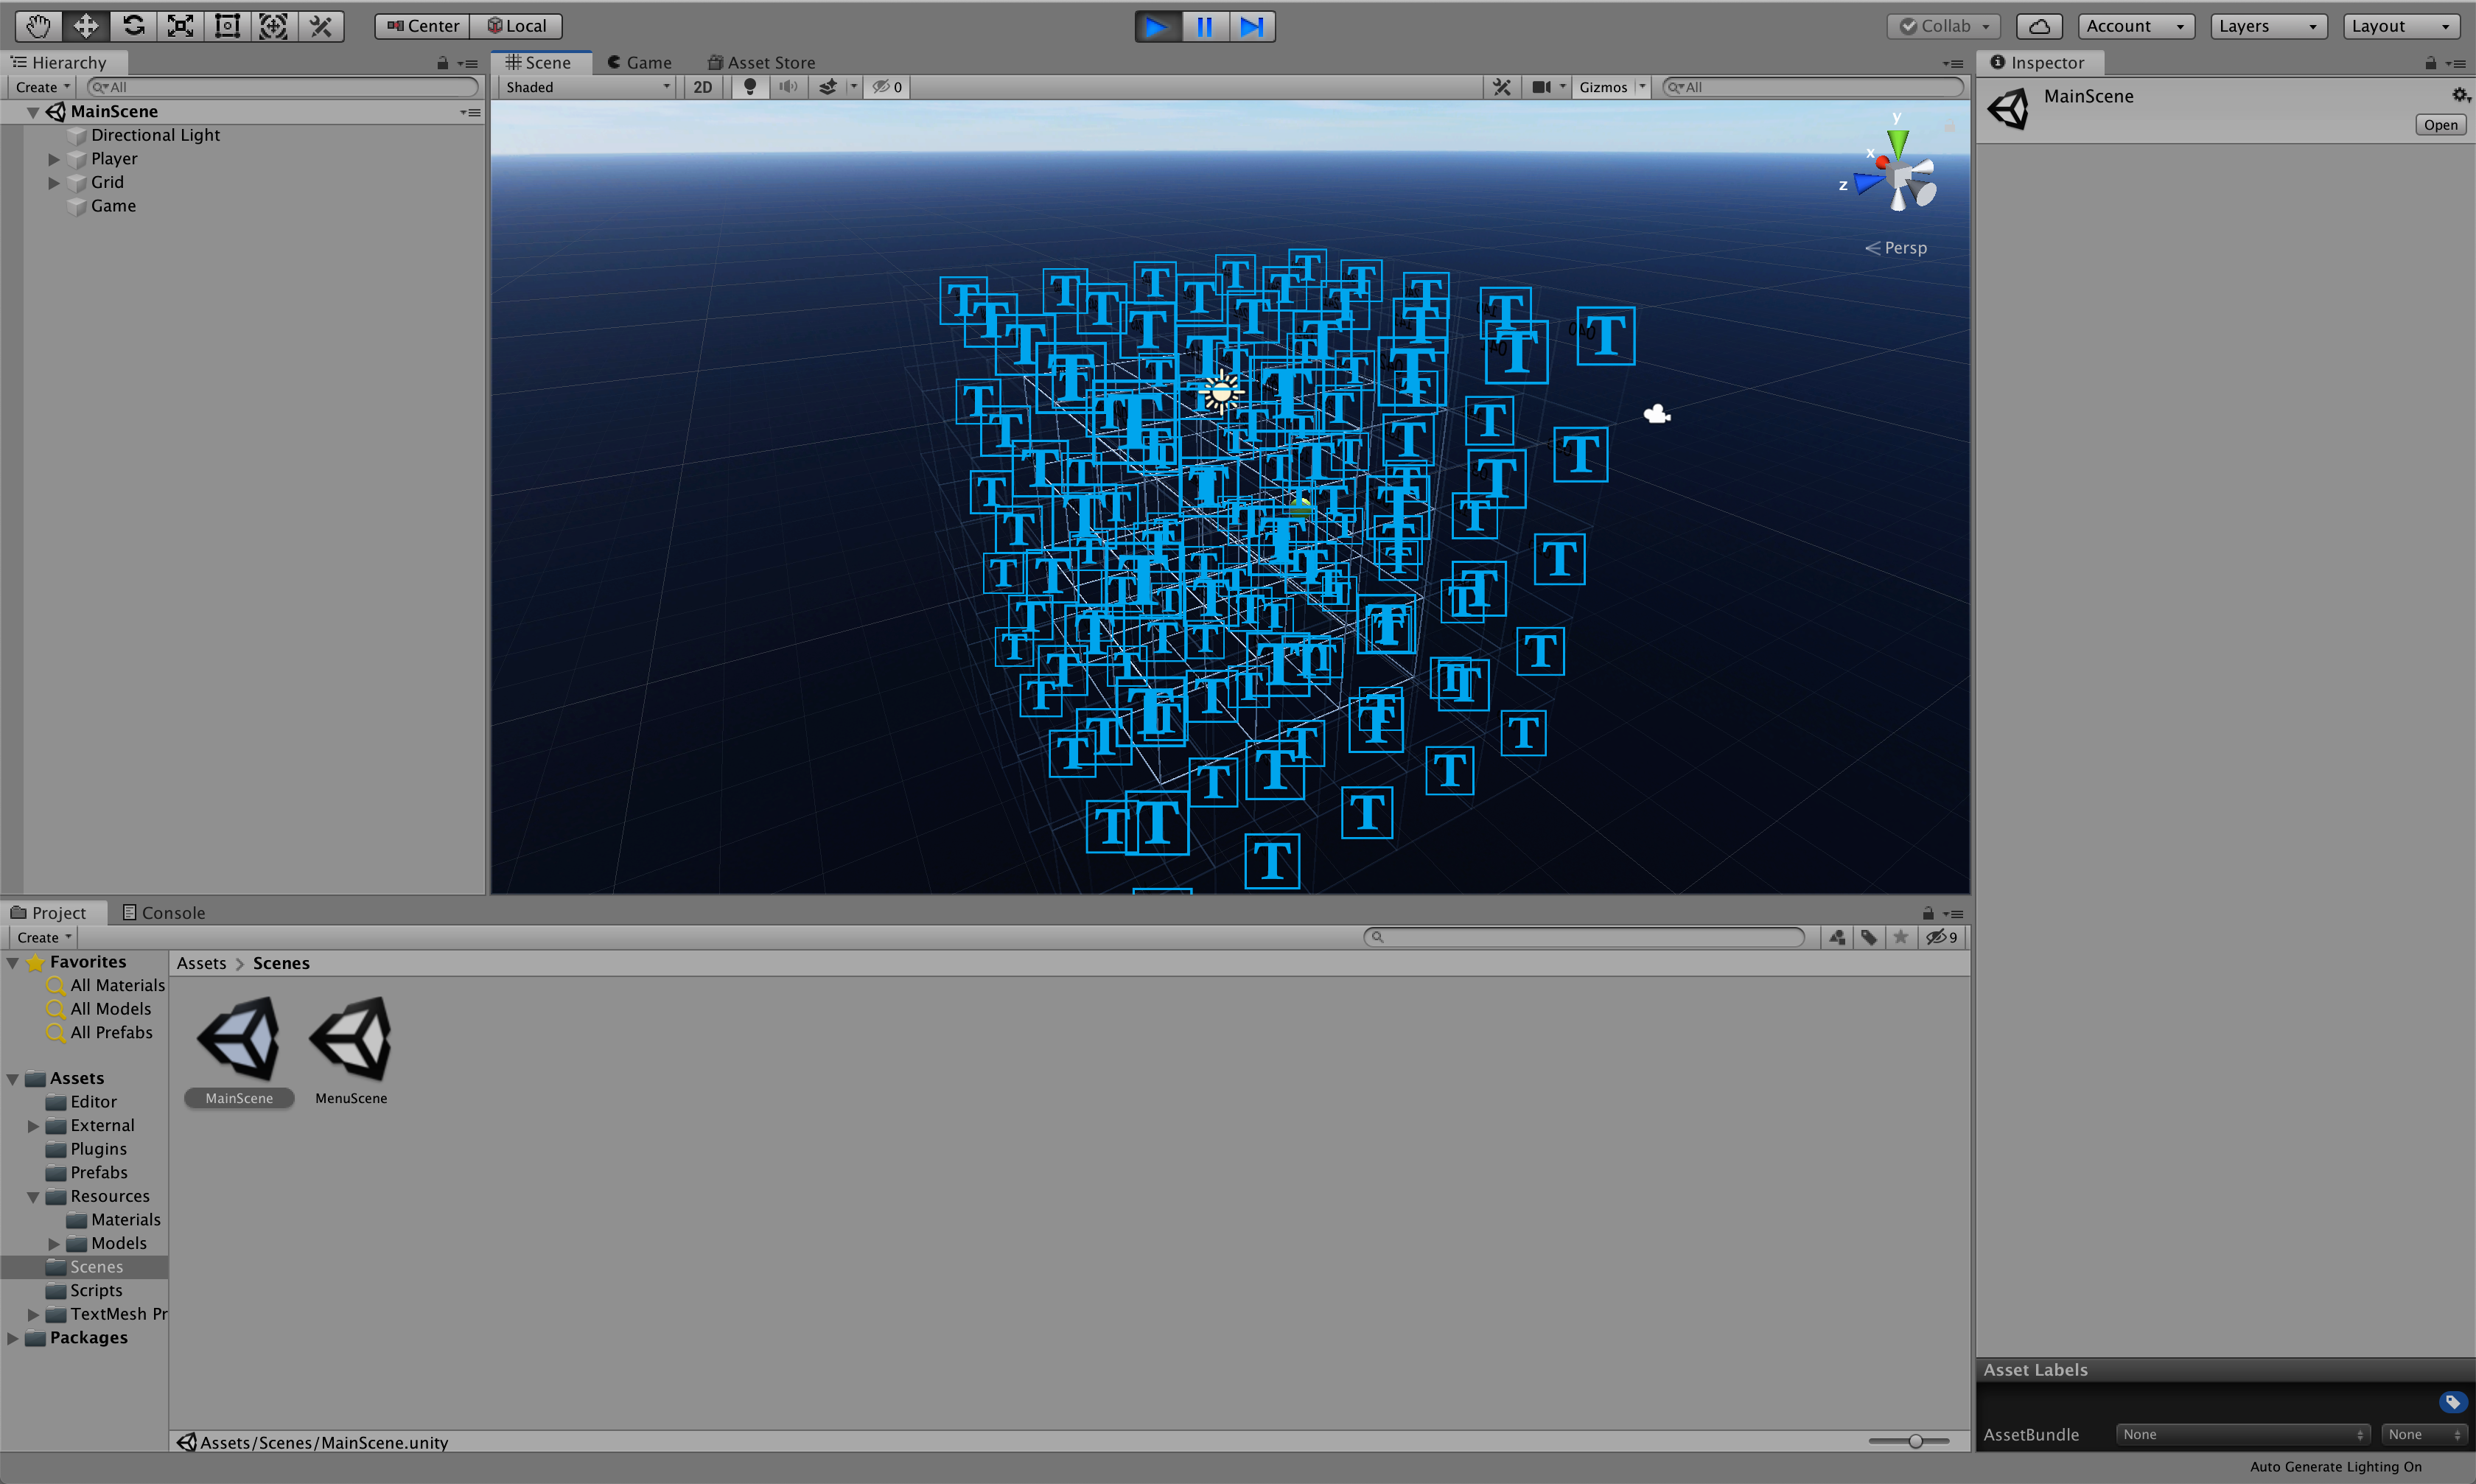
\includegraphics[width=0.8\textwidth]{images/unity.png}
    \caption{Prostredie unity}
\end{figure}\label{figure:unity}

V unity sú vstupy mapované do tzv. osí, čo dovoľuje použitie aplikácie na viacerých zariadeniach,
pričom pre všetky zariadenia existuje len jeden kód.
Napríklad pre použitie joystick-u a tlačidiel pre šípky vpravo alebo vľavo sa použije os s názvom \enquote{Horizontal},
ktorej hodnota je -1 v prípade, že užívateľ posunie joystick vľavo, resp. stlačí ľavú šípku a hodnota je 1 v prípade,
že užívateľ posunie joystick vpravo, resp. stlačí pravú šípku.
Pomocou týchto osí je možná napr. navigácia v hlavnom menu alebo otáčanie hracieho priestoru.

\subsubsection{Prostredie Cave}
Cave (z angl. \textbf{C}ave \textbf{a}utomatic \textbf{v}irtual \textbf{e}nvironment) prostredie je také, ktoré
zobrazuje obraz na štyroch plochách súčasne.\cite{cave}
Ak pozorovateľ stojí priamo, tak jedno plátno je pred ním, ďalšie sú vpravo a vľavo kolmé na plátno pred ním a posledné
je plátno pri nohách pozorovateľa.
Projektory sú umiestnené nad celým týmto systémom a navyše sa celý obraz zobrazuje upravený pre 3D okuliare.
Systém je zobrazený na obrázku nižšie.
Unity pracuje najmä s prostredím \textbf{KAVE} (skr. Kinect Cave) a teda už z názvu vyplýva, že celý systém ovládania
je založený na zariadení Microsoft Xbox Kinect a preto aj ovládanie prebieha pomocou ovládača k zariadeniu Xbox.

\begin{figure}[H]
    \centering
    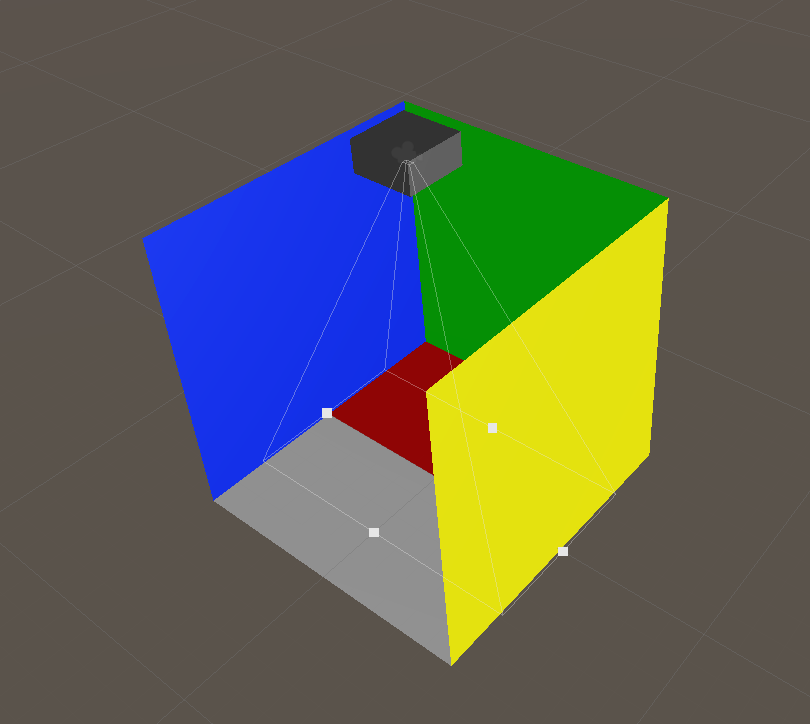
\includegraphics[width=0.4\textwidth]{images/kave.png}
    \caption{Prostredie Cave}
\end{figure}

V súvislosti s karanténou spojenou so šíriacim sa ochorením Covid-19 nebolo možné dokončiť aplikáciu v prostredí Cave,
no je plne funkčná ako desktopová aplikácia s možnosťou behu na akejkoľvek platforme (Windows, MacOS, resp. OSX aj
Linux).

\subsection{Vývojové prostriedky pre umelú inteligenciu}\label{subsec:dev-tools-for-ai}

Oba algoritmy umelej inteligencie (minimax a umelá neurónová sieť) boli implementované v jazyku Python verzie 3.7.

\subsubsection{Minimax}

Pretože samotný pseudokód algoritmu minimax je jednoduchý, aj jeho implementácia je triviálna:
\begin{figure}[H]
    \centering
    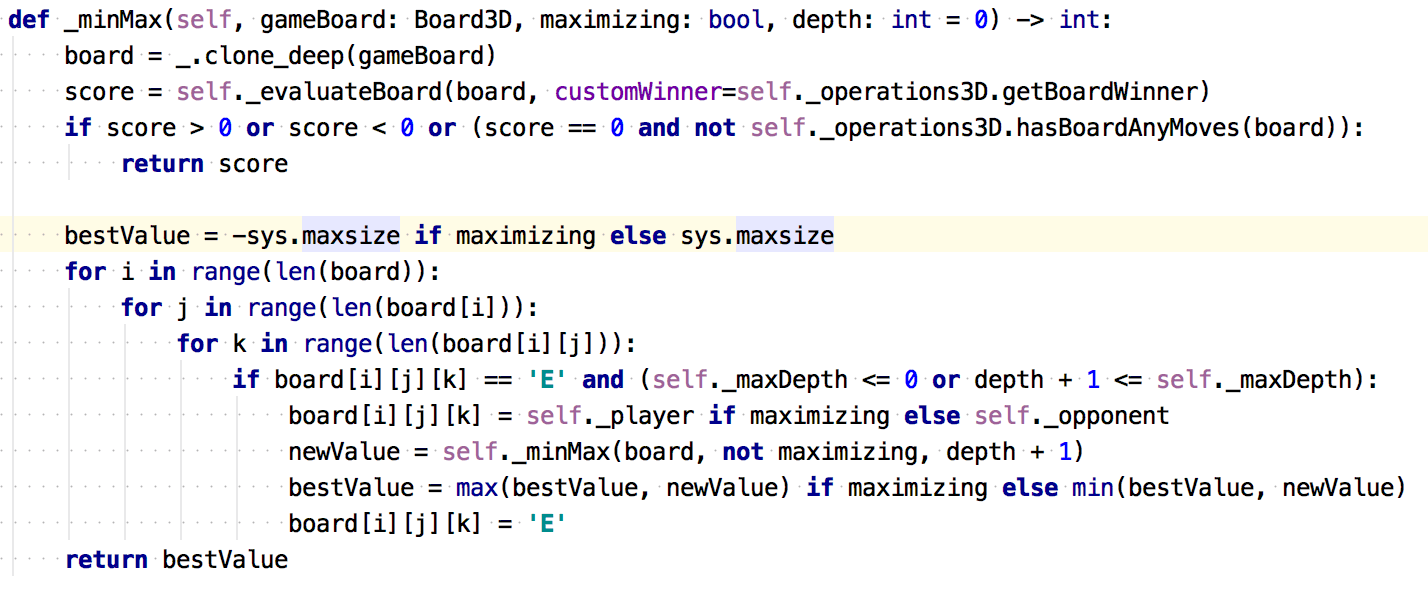
\includegraphics[width=0.8\textwidth]{images/impl-minimax.jpg}
    \caption{Implementácia algoritmu minimax}
\end{figure}\label{figure:minimax-impl}

\subsubsection{Umelá neurónová sieť}

Pre implementáciu algoritmov umelej inteligencie, existuje knižnica \emph{Tensorflow}\cite{tensorflow} od spoločnosti
Google.
Táto knižnica okrem umelých neurónových sietí ponúka aj možnosti pre implementáciu pre mnohé iné algoritmy týkajúce sa
strojového učenia.
Pre potreby umelých neurónových sietí bola vyvinutá knižnica \emph{Keras}\cite{keras}, ktorú vyvíja viac vývojárov
(no za hlavného autora je považovaný Google).
Keras umožňuje definovať štruktúru neurónovej siete, Tensorflow túto sieť natrénuje.
Okrem implementácie tried a štruktúr programu sú dôležité práve dve časti a to štruktúra umelej neurónovej siete a
trénovanie umelej neurónovej siete.

Model bol vytvorený na základe návrhu v \autoref{subsec:algo-ann} a jeho parametre boli nastavené na základe
parametrov vstupujúcich do programu.
Jedná sa teda o $3r^d$ vstupov (inputs), kde $d=3$ pretože daná sieť je implementovaná v rámci 3D priestoru a $r$ je
rovné veľkosti poľa \emph{board}.
Pole board je síce trojrozmerné, no keďže veľkosť je rovnaká v každom rozmere (kocka), stačí použiť veľkosť hlavnej
štruktúry.
Jediná skrytá vrstva má veľkosť $r^d$ a aj keď je v \autoref{subsec:algo-ann} uvedené, že na výstupe je len
jeden neurón (index s najväčšou pravdepodobnosťou výhry), knižnica Tensorflow vyžaduje aby týchto výstupov bolo $r^d$.
Dôvodom tohto prístupu je fakt, že z technického hľadiska sa jedná o \emph{klasifikáciu} (zaradenie vstupu k jednému z
výstupov).
Knižnica z $r^d$ možností pohybu hráča rozhodne o tom, ktoré políčko má pre hráča najvyššiu pravdepodobnosť výhry
pomocou tzv. \emph{one-hot array}.
Je to vektor (pole) $s_i$, ktorý má $r^d$ prvkov, $\forall i : i\neq k : s_i=0$ a $s_k=1$, kde $k$ označuje index
políčka s najpravdepodobnejším víťazstvom.
Napr. pre $r=3$, $d=3$ a $k=4$ pole vyzerá nasledovne:
\begin{equation}
    s = <0, 0, 0, 1, 0, 0, 0, 0, 0>
\end{equation}

Model je vytvorený ako sekvenčný, čo znamená, že sieť je dopredná (signál sa šíri iba smerom od vstupnej vrstvy k
výstupnej).
Všetky vrstvy v sieti sú označené ako \emph{dense}, čo vyjadruje, že všetky neuróny $i$-tej vrstvy sú prepojené so
všetkými neurónmi vrstvy $i+1$.
Všetky neuróny vstupnej a skrytej vrstvy sú aktivované pomocou funkcie \emph{ReLu} (\emph{activation=relu}), posledná
vrstva obsahuje neuróny aktivované pomocou funkcie \emph{SoftMax} (\emph{activation=softmax}).
Posledná vrstva vyžaduje túto aktivačnú funkciu, pretože výstupom z nej je klasifikácia.
Model je kompilovaný s účelovou funkciou \emph{kategorická krížová entropia} (\emph{loss=categorical\_crossentropy}).
Pri riešení minimalizačnej úlohy v rámci umelej neurónovej siete je využitý \emph{RMSProp optimizer} založený na
stochastickej gradientovej metóde (\emph{optimizer=rmsprop}).
Ukazovateľ optimality je presnosť v zaradení do jednotlivých kategórií (\emph{metrics=[acc]} - možnosť vyplniť viac
ukazovateľov).

Pre potreby trénovania je nutné pripraviť vzorku dát pre umelú neurónovú sieť.
Tieto dáta sa získavajú simulovaním náhodných hier a sú rozdelené na dáta pre hráča a dáta pre oponenta.
Dáta pre oponenta sa využívajú len pri experimentoch.
Obe tieto skupiny sú rozdelené na vstupnú časť a výstupnú časť, pričom sú rozdelené ešte na trénovaciu a testovaciu časť
v pomere 4:1 (4 trénovacie vzorky na 1 testovaciu), resp. trénovacia časť tvorí 80\% všetkých vzoriek a testovacia časť
20\%.

\begin{figure}[H]
    \centering
    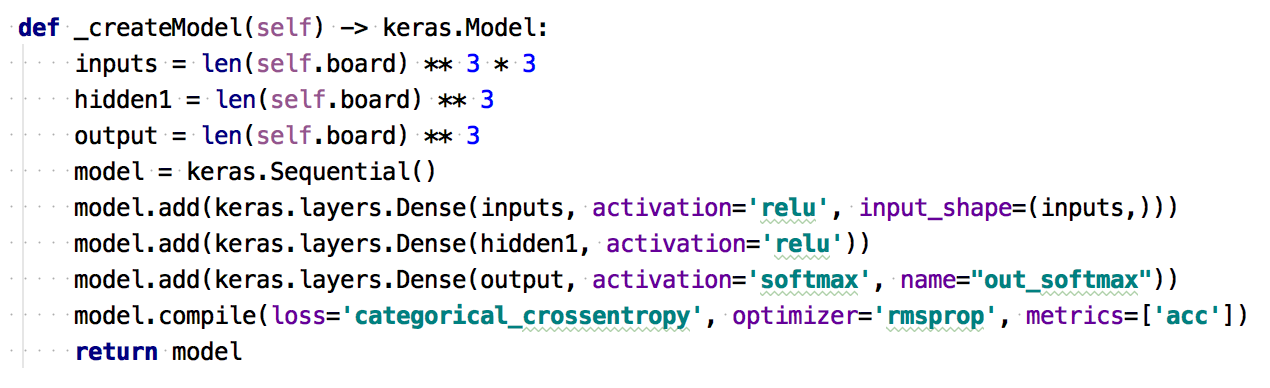
\includegraphics[width=0.8\textwidth]{images/impl-ann-model.jpg}
    \caption{Implementácia štruktúry umelej neurónovej siete}
\end{figure}\label{figure:ann-model-impl}

\begin{figure}[H]
    \centering
    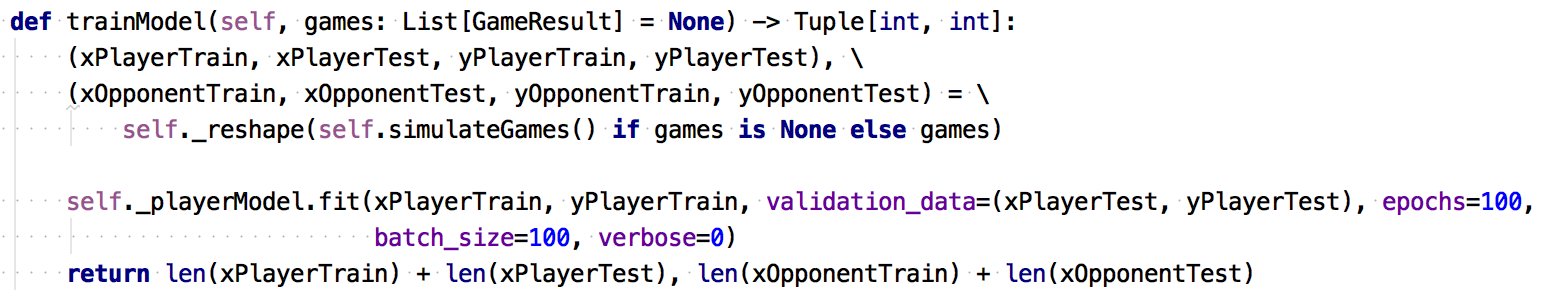
\includegraphics[width=0.8\textwidth]{images/impl-ann-train.jpg}
    \caption{Implementácia trénovania umelej neurónovej siete}
\end{figure}\label{figure:ann-train-impl}

\subsection{Prepojenie umelej inteligencie s prostredím}\label{subsec:connection}

Aby sa mohli natrénované modely využiť pre praktické použitie (v hre) je možné tieto modely uložiť na disk.
Ukladanie prebieha jednoducho zavolaním metódy \emph{save} a \emph{save\_weights} nad natrénovaným modelom a definovaním
cesty pre uložené súbory.
Následne je potrebné uložiť ešte aj celú reláciu trénovania (pomocou \emph{freeze\_session}) a nakoniec zapísať celú
štruktúru ako graf s použitím \emph{write\_graph}.
Tento graf sa do súboru uloží ako binárny súbor.
\begin{figure}[H]
    \centering
    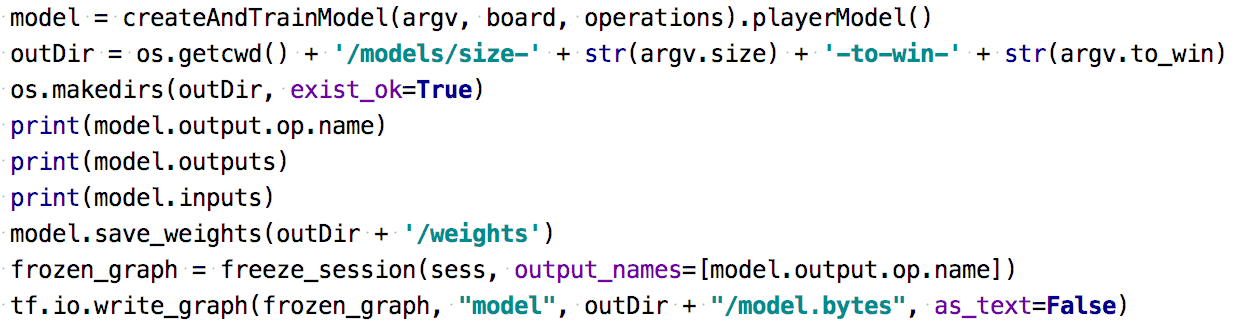
\includegraphics[width=0.8\textwidth]{images/impl-ann-save.png}
    \caption{Implementácia ukladania ANN na disk}
\end{figure}\label{figure:ann-save-impl}
Modely sa ukladajú do samostatných priečinkov pomenovaných nasledovne: \enquote{size-$r$-to-win-$w$}.
Pre použitie tejto uloženej štruktúry je možné využiť knižnicu \emph{TensorflowSharp}, ktorá je vyvinutá pre C\# a ktorá
poskytuje viac-menej tie isté možnosti ako Tensorflow pre python.
V aplikácii je použitá pre načítanie modelov z disku a ich použitie v samotnej hre.
\begin{figure}[H]
    \centering
    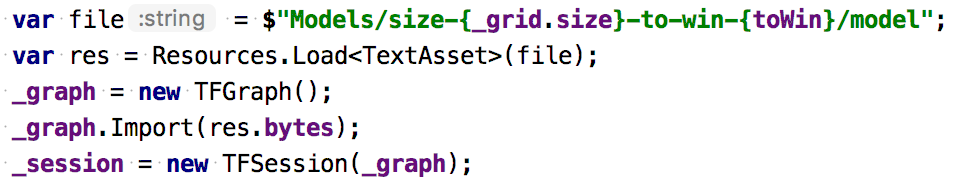
\includegraphics[width=0.8\textwidth]{images/impl-ann-load.png}
    \caption{Implementácia načítania ANN z disku}
\end{figure}\label{figure:ann-load-impl}
\begin{figure}[H]
    \centering
    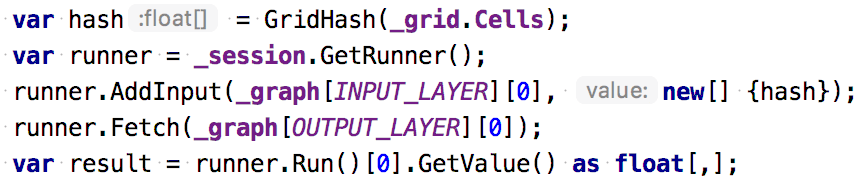
\includegraphics[width=0.8\textwidth]{images/impl-ann-usage.png}
    \caption{Implementácia použitia ANN v aplikácii}
\end{figure}\label{figure:ann-usage-impl}

\subsection{Cloud computing a automatické zostavenie}\label{subsec:ci}

Za účelom automatizácie a zrýchlenia zostavenia bol nastavený aj continuous deployment (súvislé nahrávanie, ďalej len
"CD") na \emph{GitLab-CI}.
Toto nastavenie umožňuje spustiť trénovanie umelej neurónovej siete a zostavenie aplikácie priamo na serveroch,
Konkrétne sa jedná o servery od spoločnosti \emph{Amazon} v rámci divízie \emph{Amazon web services}.
Na trénovanie ANN sa použila inštancia Linuxového serveru optimalizovaného pre lepší výkon operačnej pamäte.
Pre zostavenie unity aplikácie (s využitím natrénovanej umelej neurónovej siete) bola použitá inštancia Windows
serveru s predinštalovanou aplikáciou Unity.
\begin{figure}[H]
    \centering
    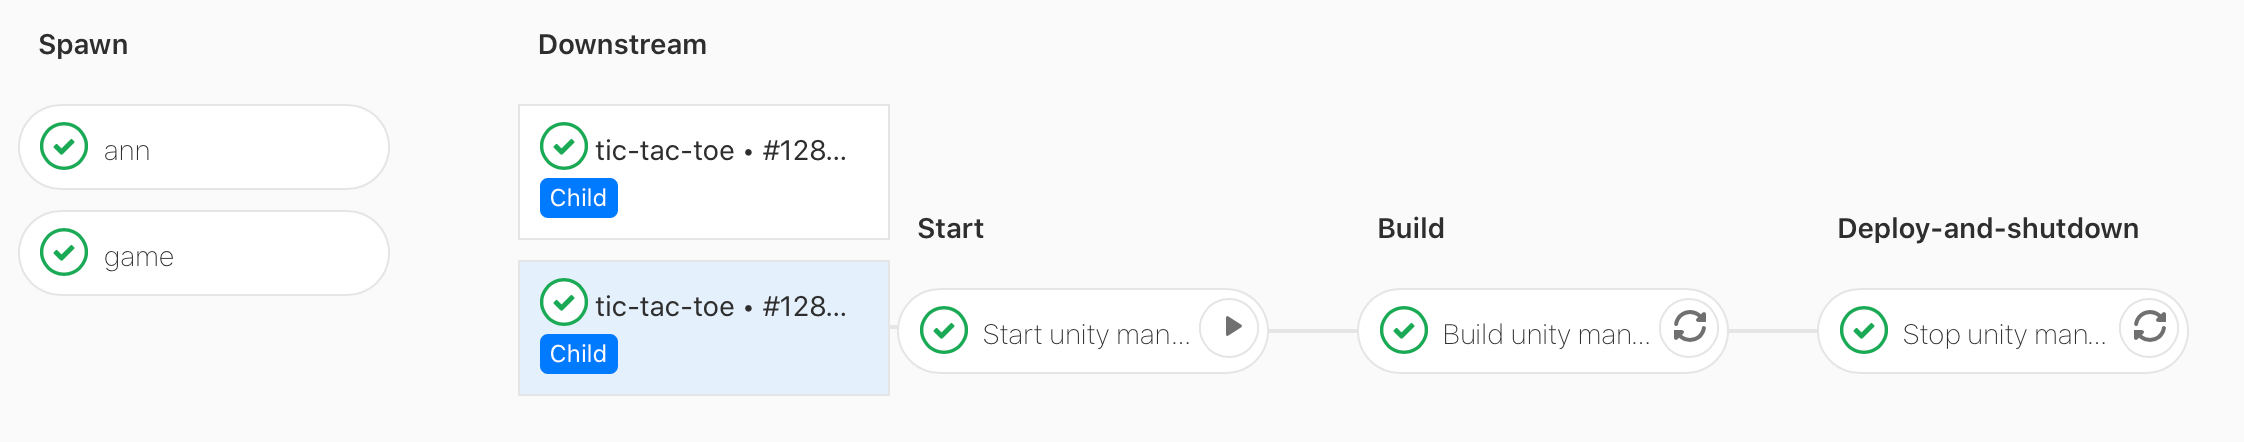
\includegraphics[width=1\textwidth]{images/impl-cd.png}
    \caption{Zobrazenie zotavenia aplikácie v rámci continuous deployment}
\end{figure}\label{figure:cd}
